\documentclass{beamer}

\usefonttheme{professionalfonts} % using non standard fonts for beamer
\usefonttheme{serif} % default family is serif

%\usepackage{hyperref}

%\usepackage{minted}

\usepackage{animate}

\usepackage{graphicx}

\def\Put(#1,#2)#3{\leavevmode\makebox(0,0){\put(#1,#2){#3}}}

\usepackage{color}

\usepackage{tikz}

\usepackage{amssymb}

\usepackage{enumerate}


\newcommand\blfootnote[1]{%

  \begingroup

  \renewcommand\thefootnote{}\footnote{#1}%

  \addtocounter{footnote}{-1}%

  \endgroup

}

\makeatletter

%%%%%%%%%%%%%%%%%%%%%%%%%%%%%% Textclass specific LaTeX commands.

 % this default might be overridden by plain title style

 \newcommand\makebeamertitle{\frame{\maketitle}}%

 % (ERT) argument for the TOC

 \AtBeginDocument{%

   \let\origtableofcontents=\tableofcontents

   \def\tableofcontents{\@ifnextchar[{\origtableofcontents}{\gobbletableofcontents}}

   \def\gobbletableofcontents#1{\origtableofcontents}

 }

%%%%%%%%%%%%%%%%%%%%%%%%%%%%%% User specified LaTeX commands.

\usetheme{Malmoe}

% or ...

\useoutertheme{infolines}

\addtobeamertemplate{headline}{}{\vskip2pt}



\setbeamercovered{transparent}

% or whatever (possibly just delete it)

\makeatother

\begin{document}
\title[SDCEL report]{Geoinformatica paper extension}
\author[AC]{}
\institute[UCR]{University of California, Riverside}
\makebeamertitle
\newif\iflattersubsect

% \AtBeginSection[] {
%   \begin{frame}<beamer>
%     \frametitle{Outline} 
%     \tableofcontents[currentsection]  
%   \end{frame}
%   \lattersubsectfalse
% }

\AtBeginSubsection[] {
  \begin{frame}<beamer>
    \frametitle{Outline} 
    \tableofcontents[currentsubsection]  
  \end{frame}
}


\begin{frame}{Kdtree vs Quadtree experiments...}{CA Dataset - Tree creation}
  \centering 
  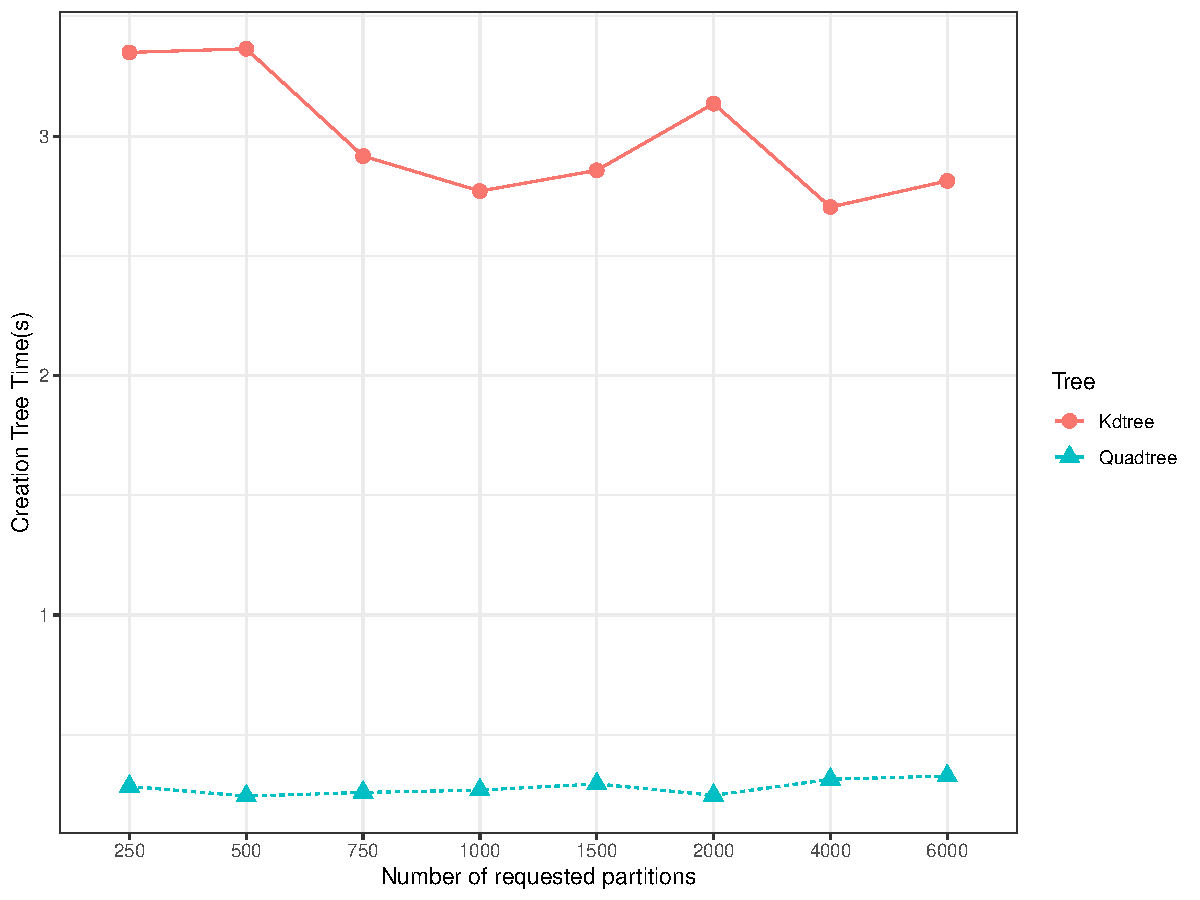
\includegraphics[width=0.7\textwidth]{figures/CA3_KdtreeVsQuadtree_Creation}
\end{frame}
\begin{frame}{Kdtree vs Quadtree experiments...}{CA Dataset - Data partitioning}
  \centering
  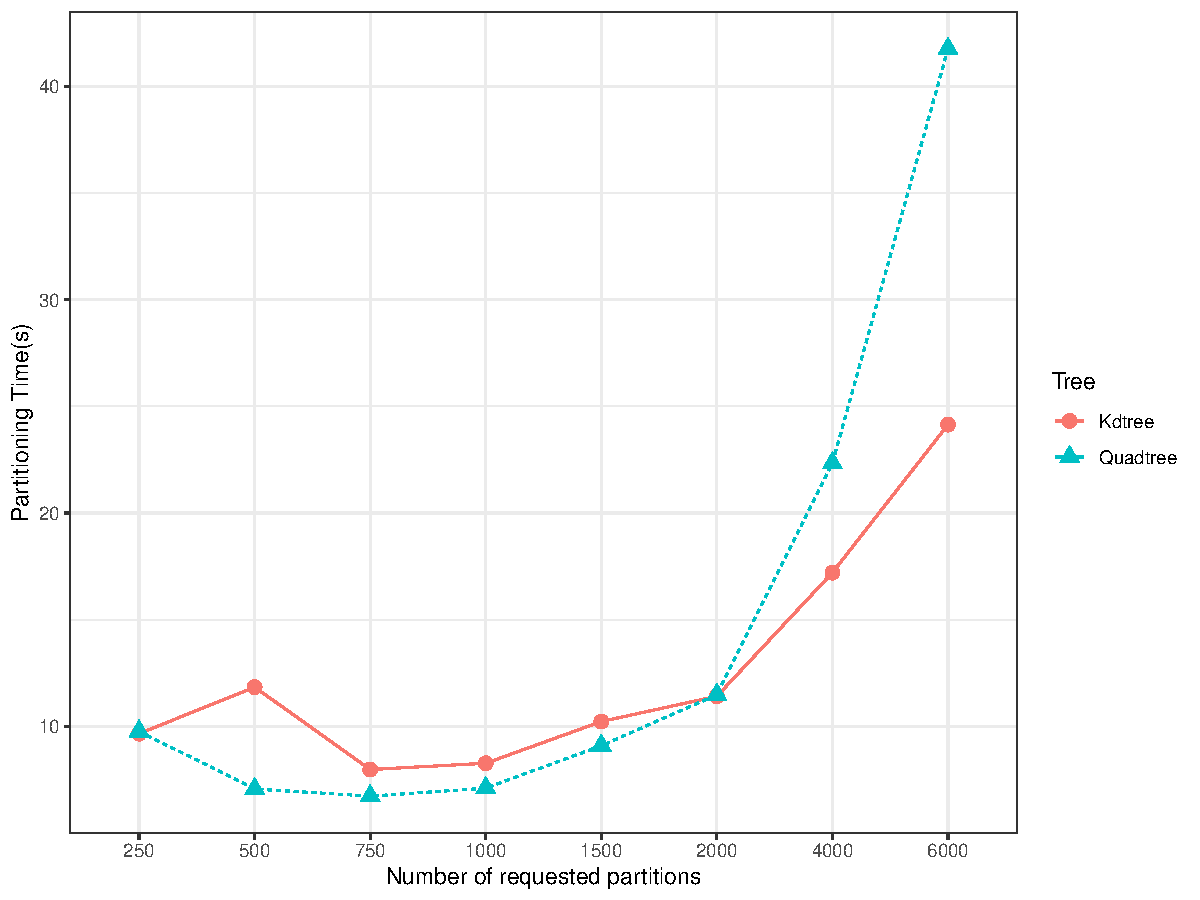
\includegraphics[width=0.7\textwidth]{figures/CA3_KdtreeVsQuadtree_Partitioning}
\end{frame}
\begin{frame}{Kdtree vs Quadtree experiments...}{CA Dataset - Layer overlay}
  \centering
  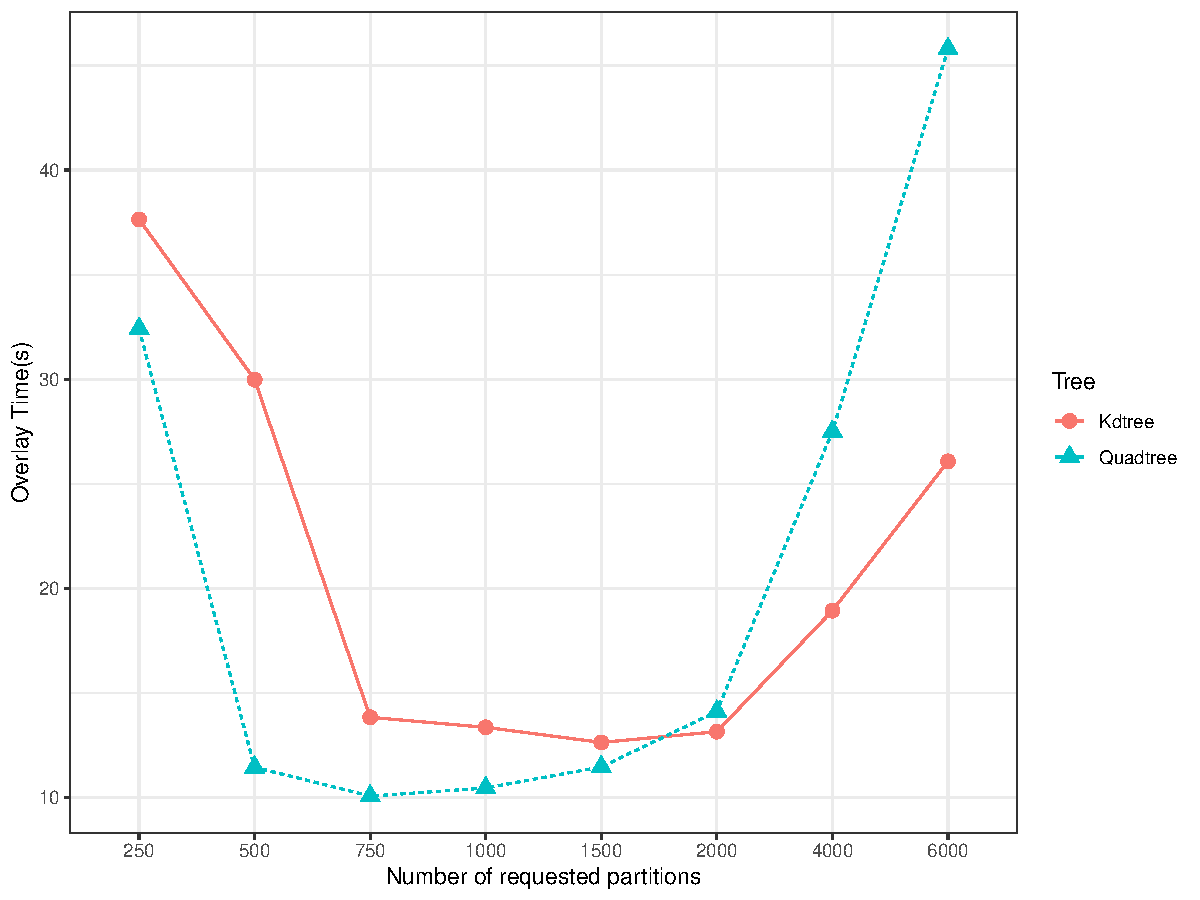
\includegraphics[width=0.7\textwidth]{figures/CA3_KdtreeVsQuadtree_Overlay}
\end{frame}
\begin{frame}{Kdtree vs Quadtree experiments...}{CA Dataset - Space}
  \centering
  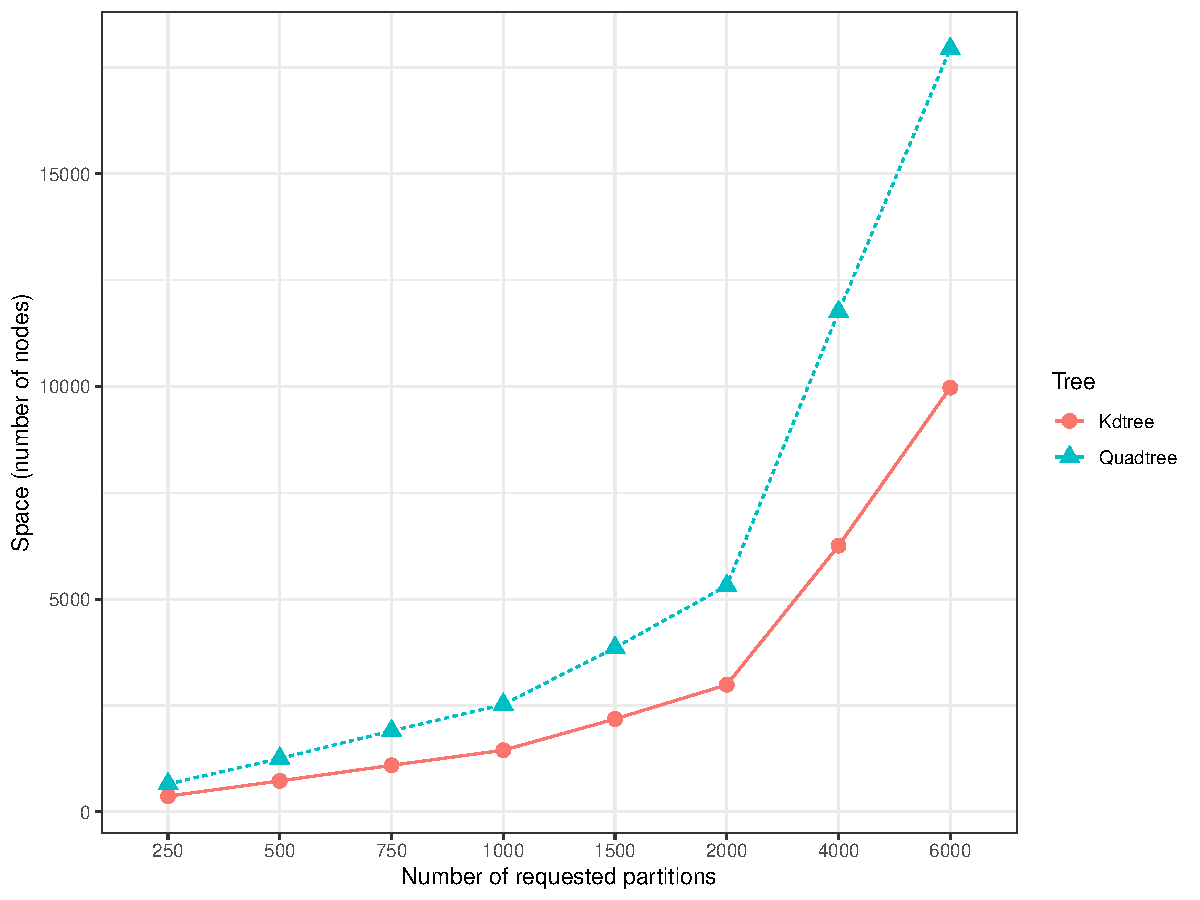
\includegraphics[width=0.7\textwidth]{figures/CA3_KdtreeVsQuadtree_Space}
\end{frame}

\begin{frame}{Kdtree vs Quadtree experiments...}{US Dataset - Tree creation}
  \centering
  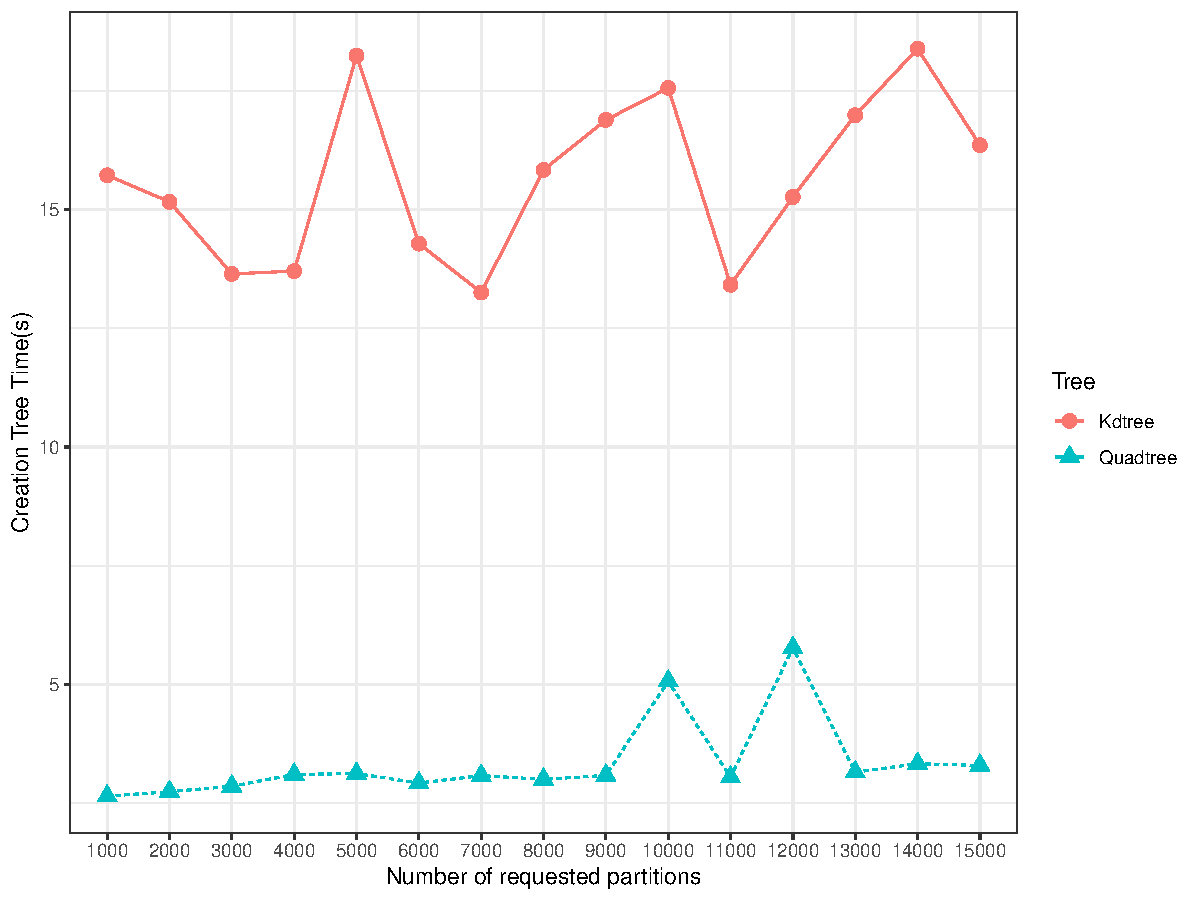
\includegraphics[width=0.7\textwidth]{figures/US_KdtreeVsQuadtree_Creation}
\end{frame}
\begin{frame}{Kdtree vs Quadtree experiments...}{US Dataset - Data partitioning}
  \centering
  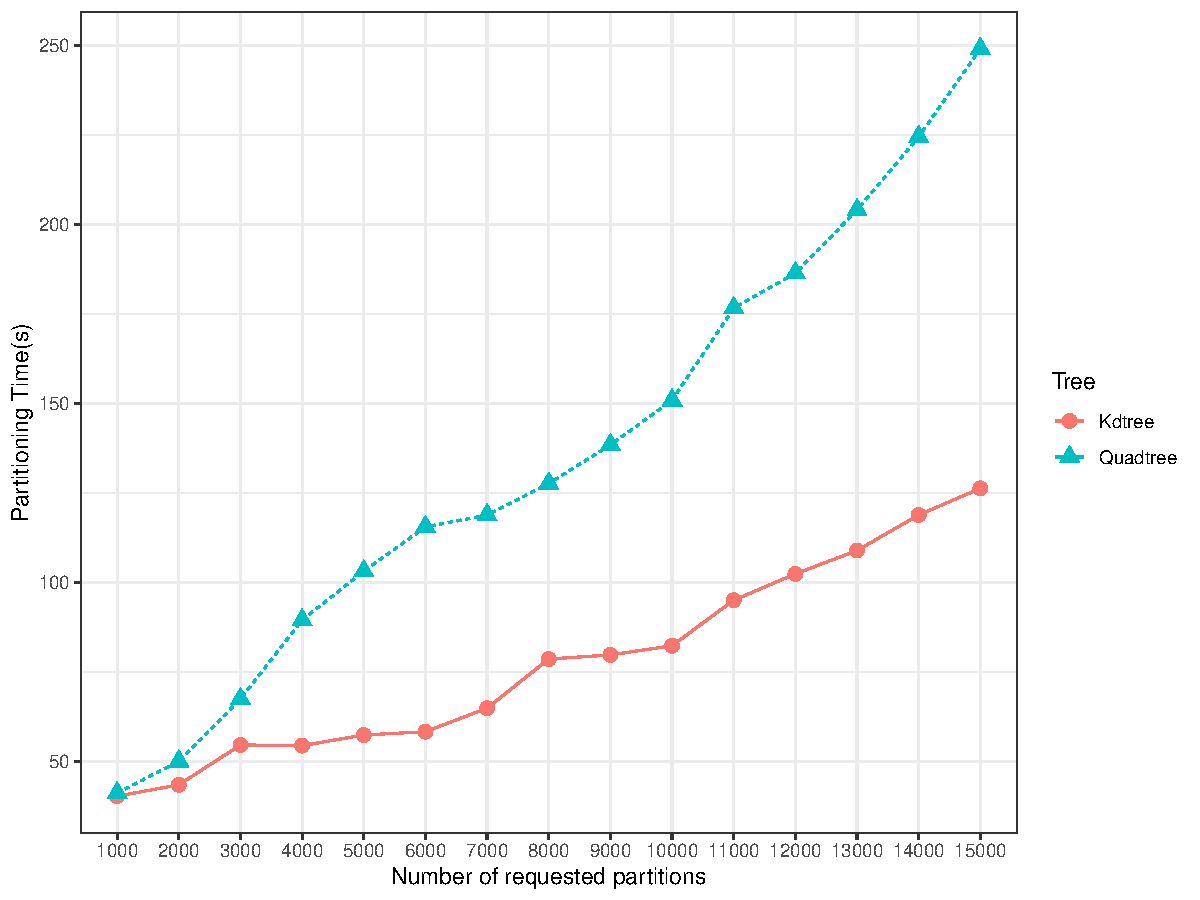
\includegraphics[width=0.7\textwidth]{figures/US_KdtreeVsQuadtree_Partitioning}
\end{frame}
\begin{frame}{Kdtree vs Quadtree experiments...}{US Dataset - Layer overlay}
  \centering
  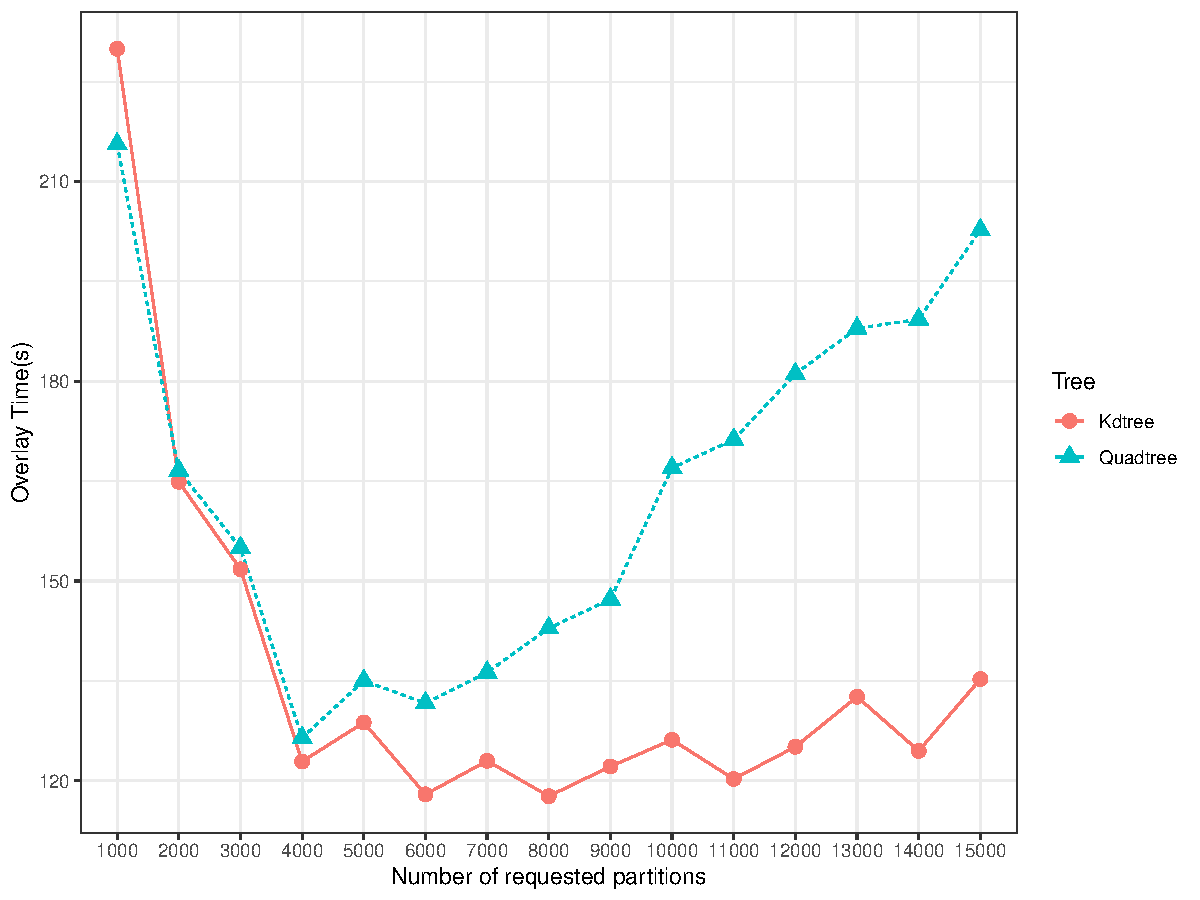
\includegraphics[width=0.7\textwidth]{figures/US_KdtreeVsQuadtree_Overlay}
\end{frame}
\begin{frame}{Kdtree vs Quadtree experiments...}{US Dataset - Space}
  \centering
  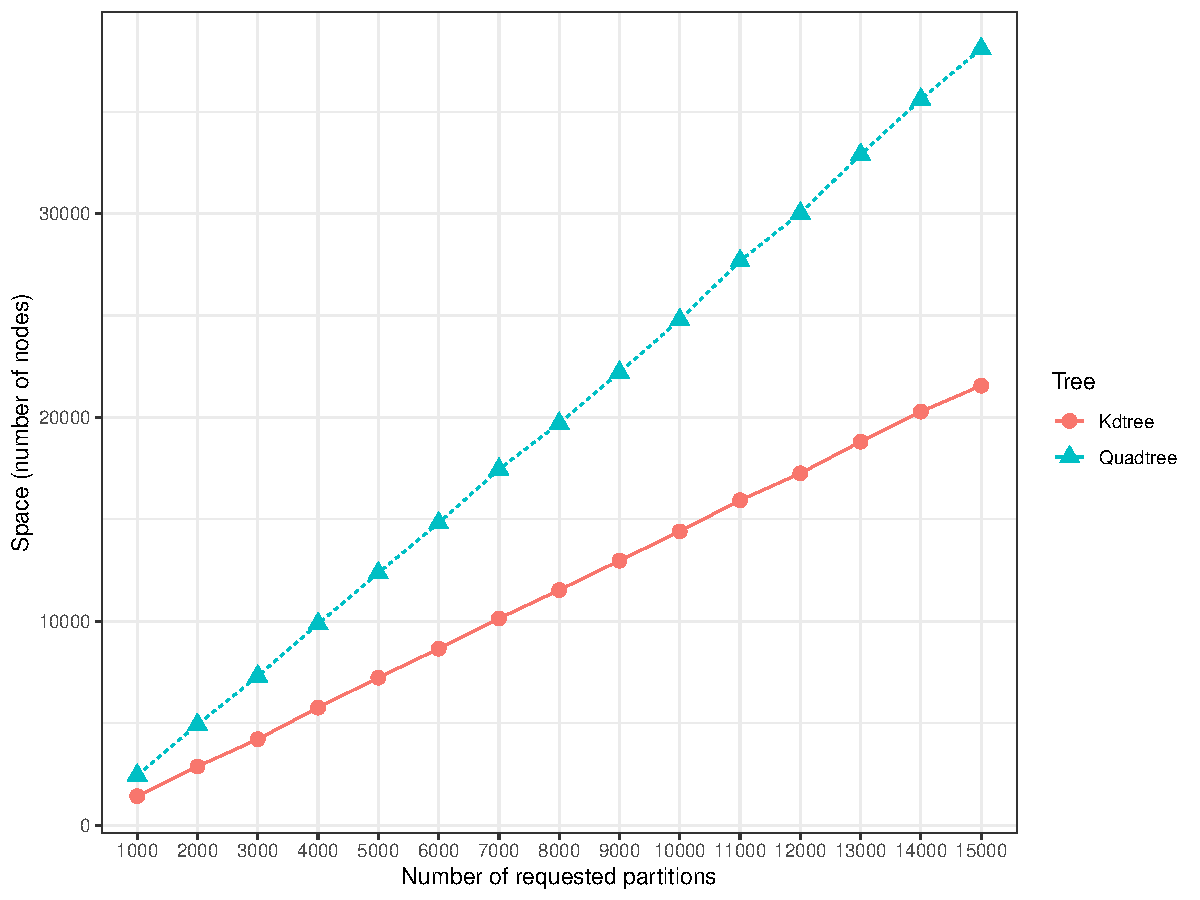
\includegraphics[width=0.7\textwidth]{figures/US_KdtreeVsQuadtree_Space}
\end{frame}

\begin{frame}{Kdtree orphan holes proposal...}
  \centering
  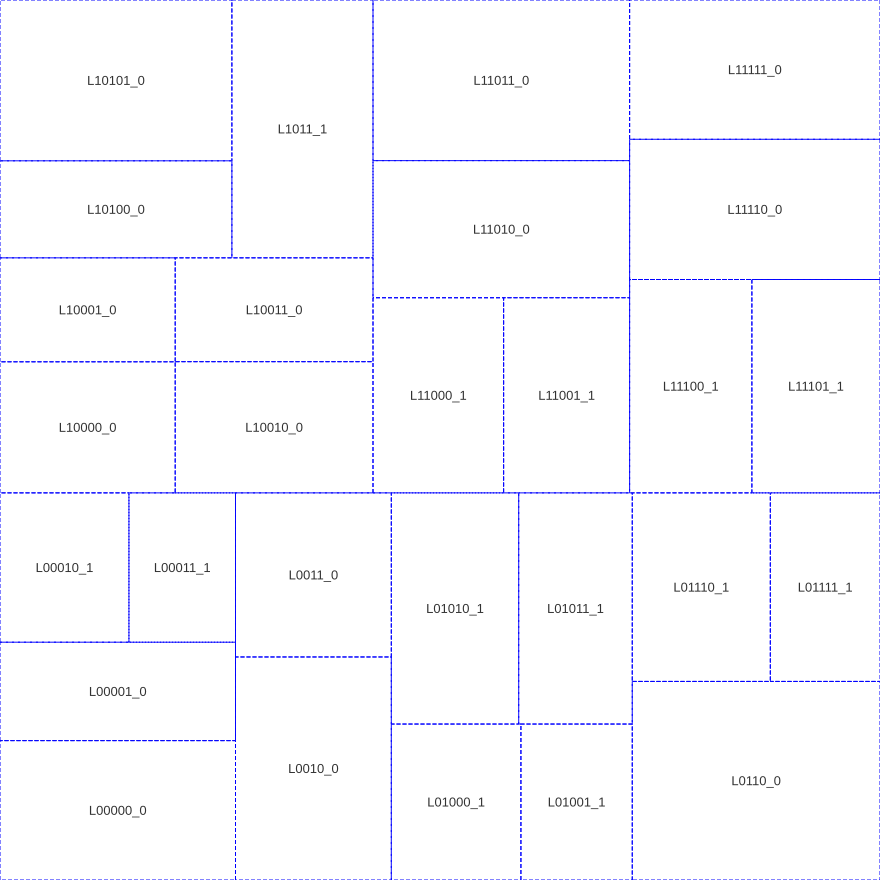
\includegraphics[width=0.6\textwidth]{figures/kdtree_lineage}
\end{frame}
\begin{frame}{Kdtree orphan holes proposal...}
  \centering
  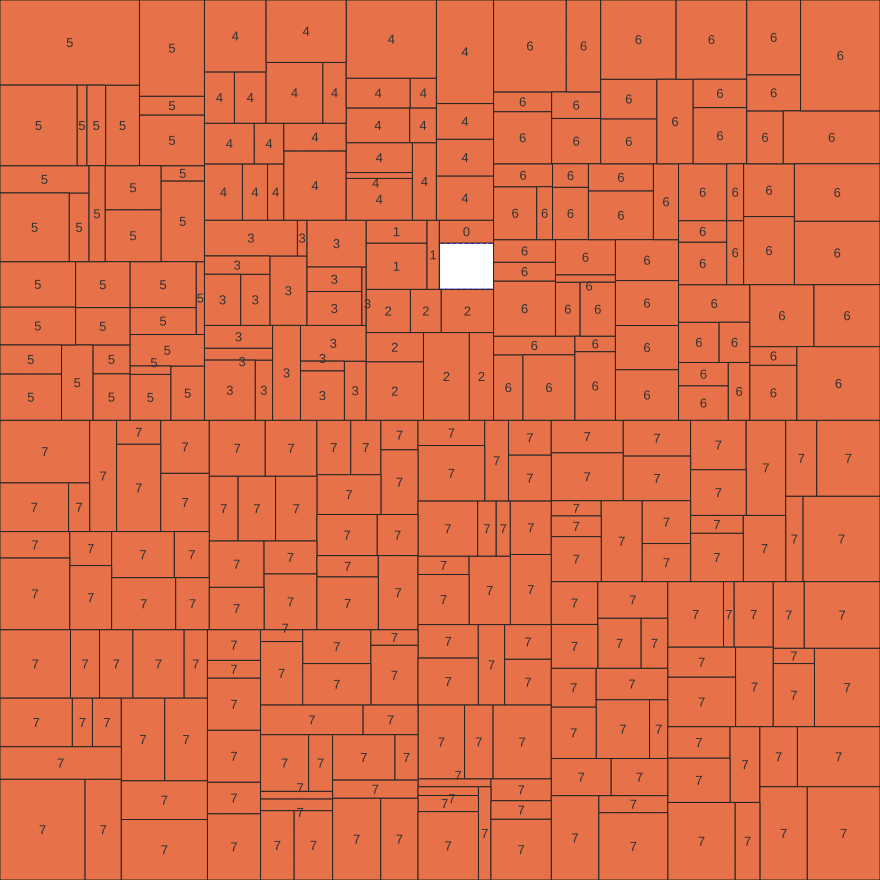
\includegraphics[width=0.6\textwidth]{figures/kdtree_ordering}
\end{frame}


%\begin{frame}{Some invalids polygons...}
%    \centering 
    %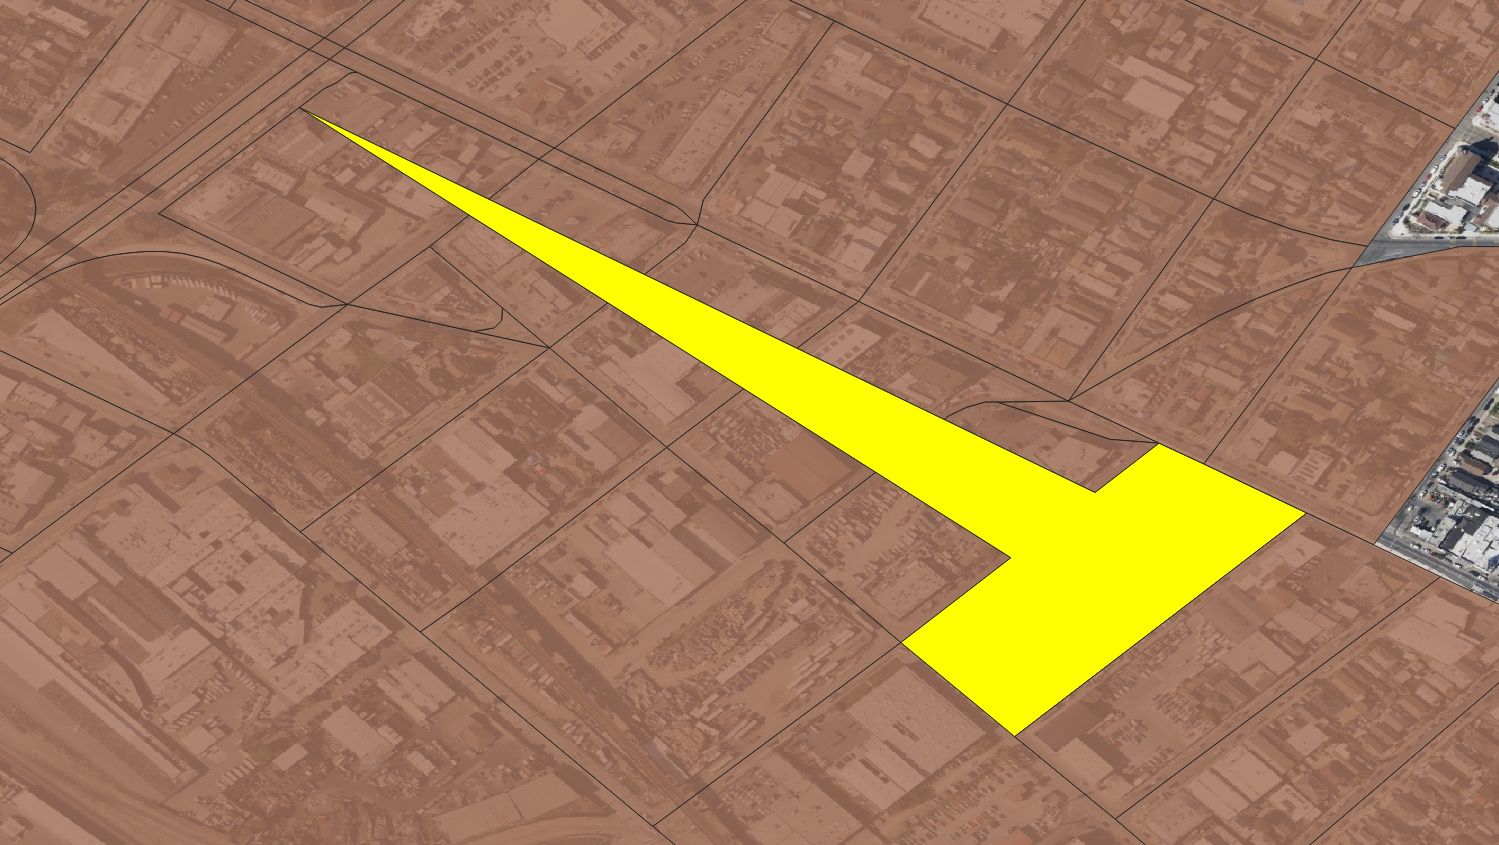
\includegraphics[width=0.8\textwidth]{figures/artifact02}
%\end{frame}

\end{document}
